% !TEX TS-program = xelatex
% !TEX encoding = UTF-8 Unicode
% !Mode:: "TeX:UTF-8"

\documentclass{resume}
\usepackage{zh_CN-Adobefonts_external} % Simplified Chinese Support using external fonts (./fonts/zh_CN-Adobe/)
% \usepackage{NotoSansSC_external}
\usepackage{NotoSerifCJKsc_external}
% \usepackage{zh_CN-Adobefonts_internal} % Simplified Chinese Support using system fonts
\usepackage{linespacing_fix} % disable extra space before next section
\usepackage{cite}
\usepackage{graphicx}
\usepackage{tabu}
\usepackage{multirow}
\usepackage{progressbar}

\begin{document}
\pagenumbering{gobble} % suppress displaying page number

\begin{center}
\Huge{个~~~人~~~简~~~历}
\end{center}
\Large{
  \begin{tabu}{ c l l }
   \multirow{5}{1in}{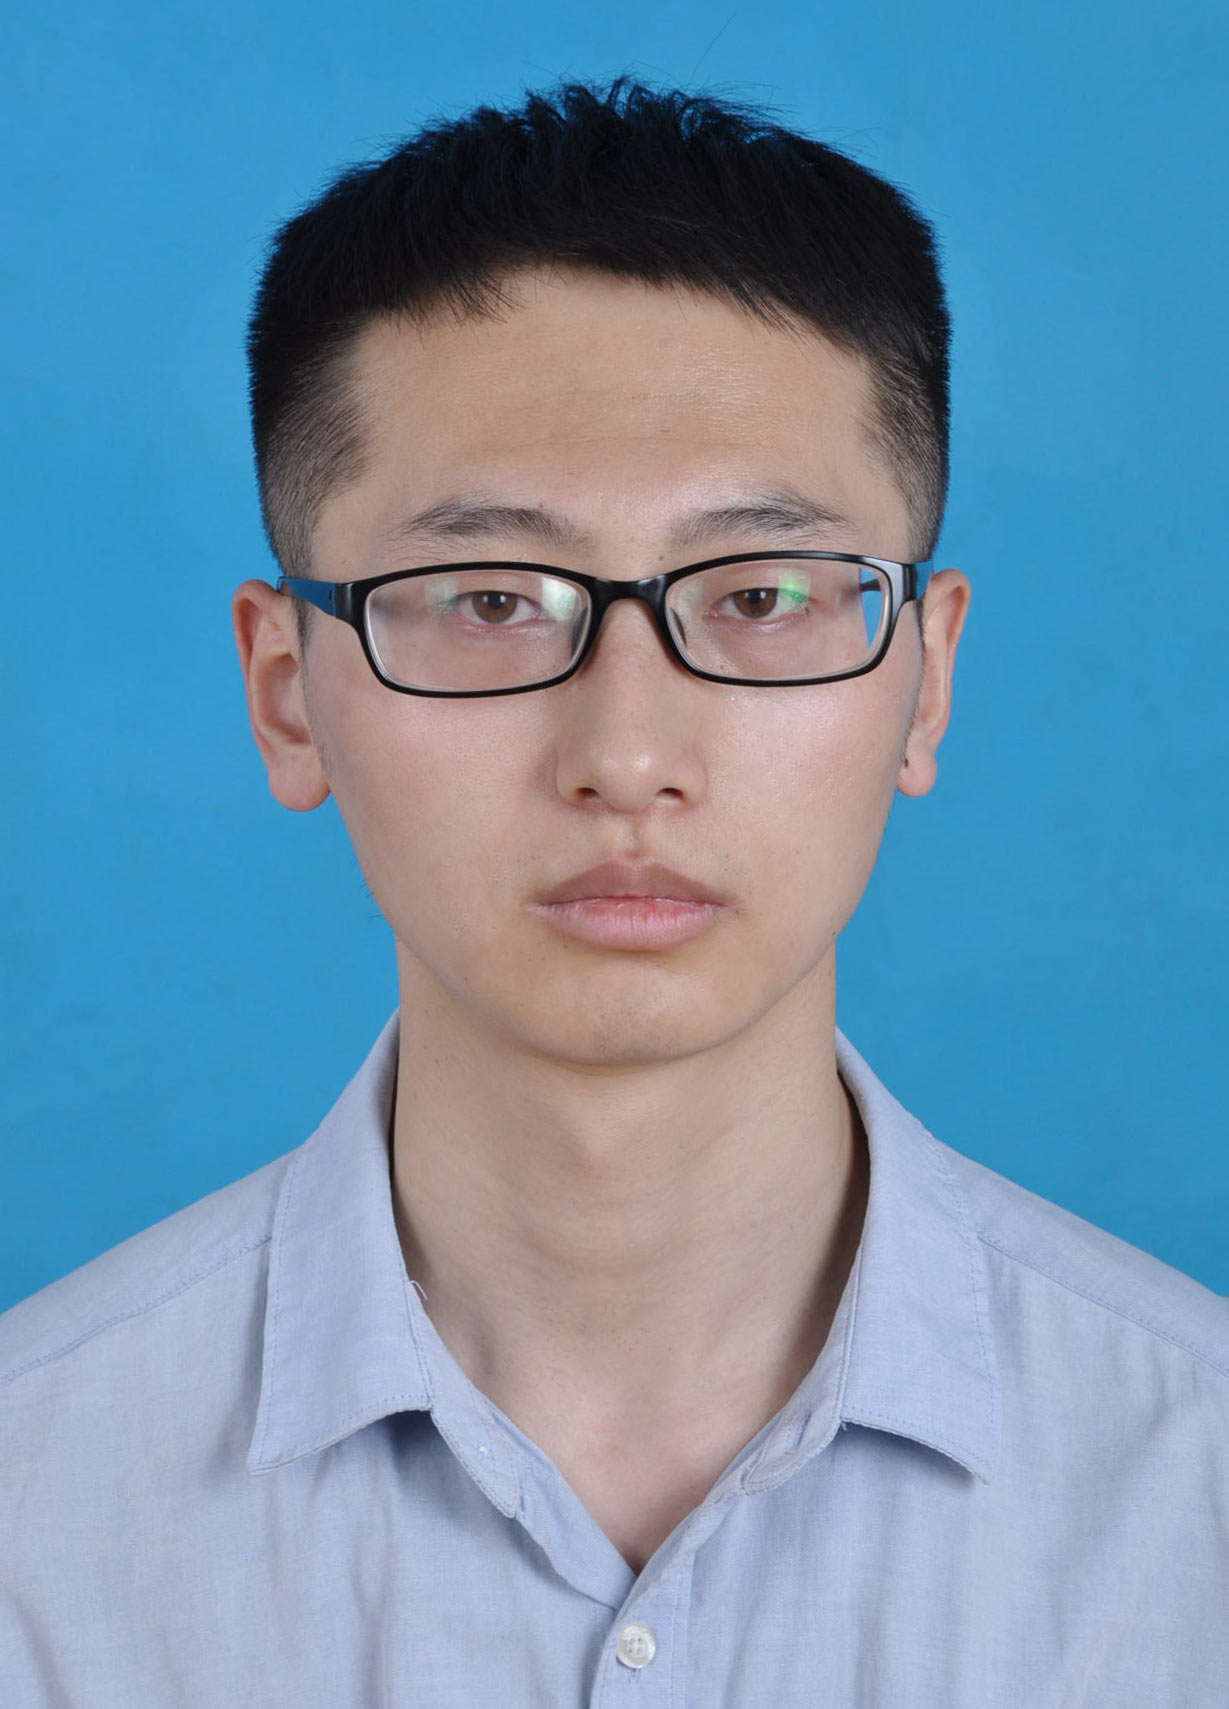
\includegraphics[width=0.88in]{avatar}} &
   \scshape{李高阳} &  \\
    & 性别:男 & 民族:汉 \\
    & 电话:(+86) 15002555080 & 生日:1991-09 \\
    & 邮箱:li.gaoyang@foxmail.com & 微信:sandbox\_ligy\\
    % & 地址:甘肃省兰州市天水南路222号 \hspace{40} & %籍贯:甘肃宁县
    & 籍贯:甘肃宁县 & 政治面貌:党员
  \end{tabu}
}

\section{教育经历}
% \textbf{兰州大学}
\datedsubsection{\textbf{兰州大学与中科院兰州近物所联合培养博士}}{2015 -- 2019}
\textit{专业:物理学\ 理论物理\qquad\qquad\qquad 研究方向:凝聚态理论}\\
\textit{导师:罗洪刚教授(长江学者)、房铁峰教授}\\
\textit{研究内容:强关联量子系统的数值重整化群研究}
\datedsubsection{\textbf{兰州大学\ 硕士}}{2013 --  2015}
\textit{专业:物理学\ 理论物理\qquad\qquad\qquad 研究方向:凝聚态理论}
\datedsubsection{\textbf{兰州大学\ 本科}}{2009 --  2013}
\textit{专业:物理学国家基地班}

\section{发表文章}
\textbf{Gao-Yang Li}, Tie-Feng Fang, Ai-Min Guo, and Qing-Feng Sun \textit{Ferromagnetism-induced Kondo effect in graphene with a magnetic impurity}, Phys. Rev. B \textbf{100}, 115115 (2019). 第一作者,SCI二区
\item Wan-Xiu He, Zhan Cao, \textbf{Gao-Yang Li}, Lin Li, Hai-Feng Lü, ZhenHua Li, and Hong-Gang Luo \textit{Performance of the T-matrix based master equation for Coulomb drag in double quantum dots}, Phys. Rev. B \textbf{101}, 035417 (2020). 第三作者,SCI二区

\section{毕业论文题目}
铁磁石墨烯中近藤效应的数值重整化群研究

\section{获奖情况}
\datedline{\textit{国家励志奖学金}}{2010 -- 2011}
\datedline{\textit{学校三等奖学金}}{2013 -- 2018}
% \datedline{其他奖项}{2015}

\section{主要课程}
力学、理论力学、电磁学、电动力学、量子力学、热力学统计物理、量子统计物理学、数学物理方法等

\section{其他技能}
% increase linespacing [parsep=0.5ex]
\begin{itemize}%[parsep=0.5ex]
% \item 能高效使用Shell脚本,有六年的Linux使用经验,并熟悉Python等
\item 英语六级,能流利进行口头交流
% \item 平常编写代码要求尽量高效、美观,并用git管理代码
% \item 自学能力强,对新知识有较高的学习热情,并能投入精力解决问题
% \item 自学了机器学习的基本知识
% \item 了解精确对角化、密度矩阵重整化群、蒙特卡罗、张量网络重整化群等数值计算方法
% \item 喜欢打羽毛球
\item 本科学习成绩在专业前30\%
% \item 对机器学习感兴趣,正在自学TensorFlow框架
\end{itemize}

% \section{自我评价}
% \qquad 自认为是一个上进努力有责任心的人,能和周围的人和睦相处,进行高效的交流。自学能力强,对新知识有较高的学习热情,能够自驱地学习需要的知识,并能投入精力解决问题。

% \section{个人主页}
% \rm{https://github.com/GoldenRaven}

%% Reference
% \newpage
% \bibliographystyle{IEEETran} \bibliography{mycite}
\end{document}
